\section{Absolute Value Functions}

\begin{definition}[Absolute Value]
    The \textbf{absolute value} of a real numberf $x$, denoted by $|x|$, is given by
    \[|x| = \begin{cases}
            -x & \text{if } x<0     \\
            x  & \text{if } x\geq 0
        \end{cases}
    \]
\end{definition}

\begin{definition}[Properties of Absolut Value]
    Let $a$, $b$ and  $x$ be real numbers and let $n$ be an integer. Then
    \begin{itemize}
        \item \textbf{Product Rule}: $|ab|= |a||b|$
        \item \textbf{Power Rule}: $|a^n| = |a|^n$ whenever $a^n$ is defined
        \item \textbf{Quotient Rule}: $|\frac{a}{b}| = \frac{|a|}{|b|}$, provided $b \neq 0$
    \end{itemize}
    \textbf{Equality Properties}:
    \begin{itemize}
        \item $|x|=0$ if and only if $x=0$.
        \item For $c>0$, $|x|=c$ if and only if $x=c$ or $-x=c$.
        \item For $c<0$, $|x|=c$ has no solution.
    \end{itemize}
\end{definition}

\subsection{Exercises}
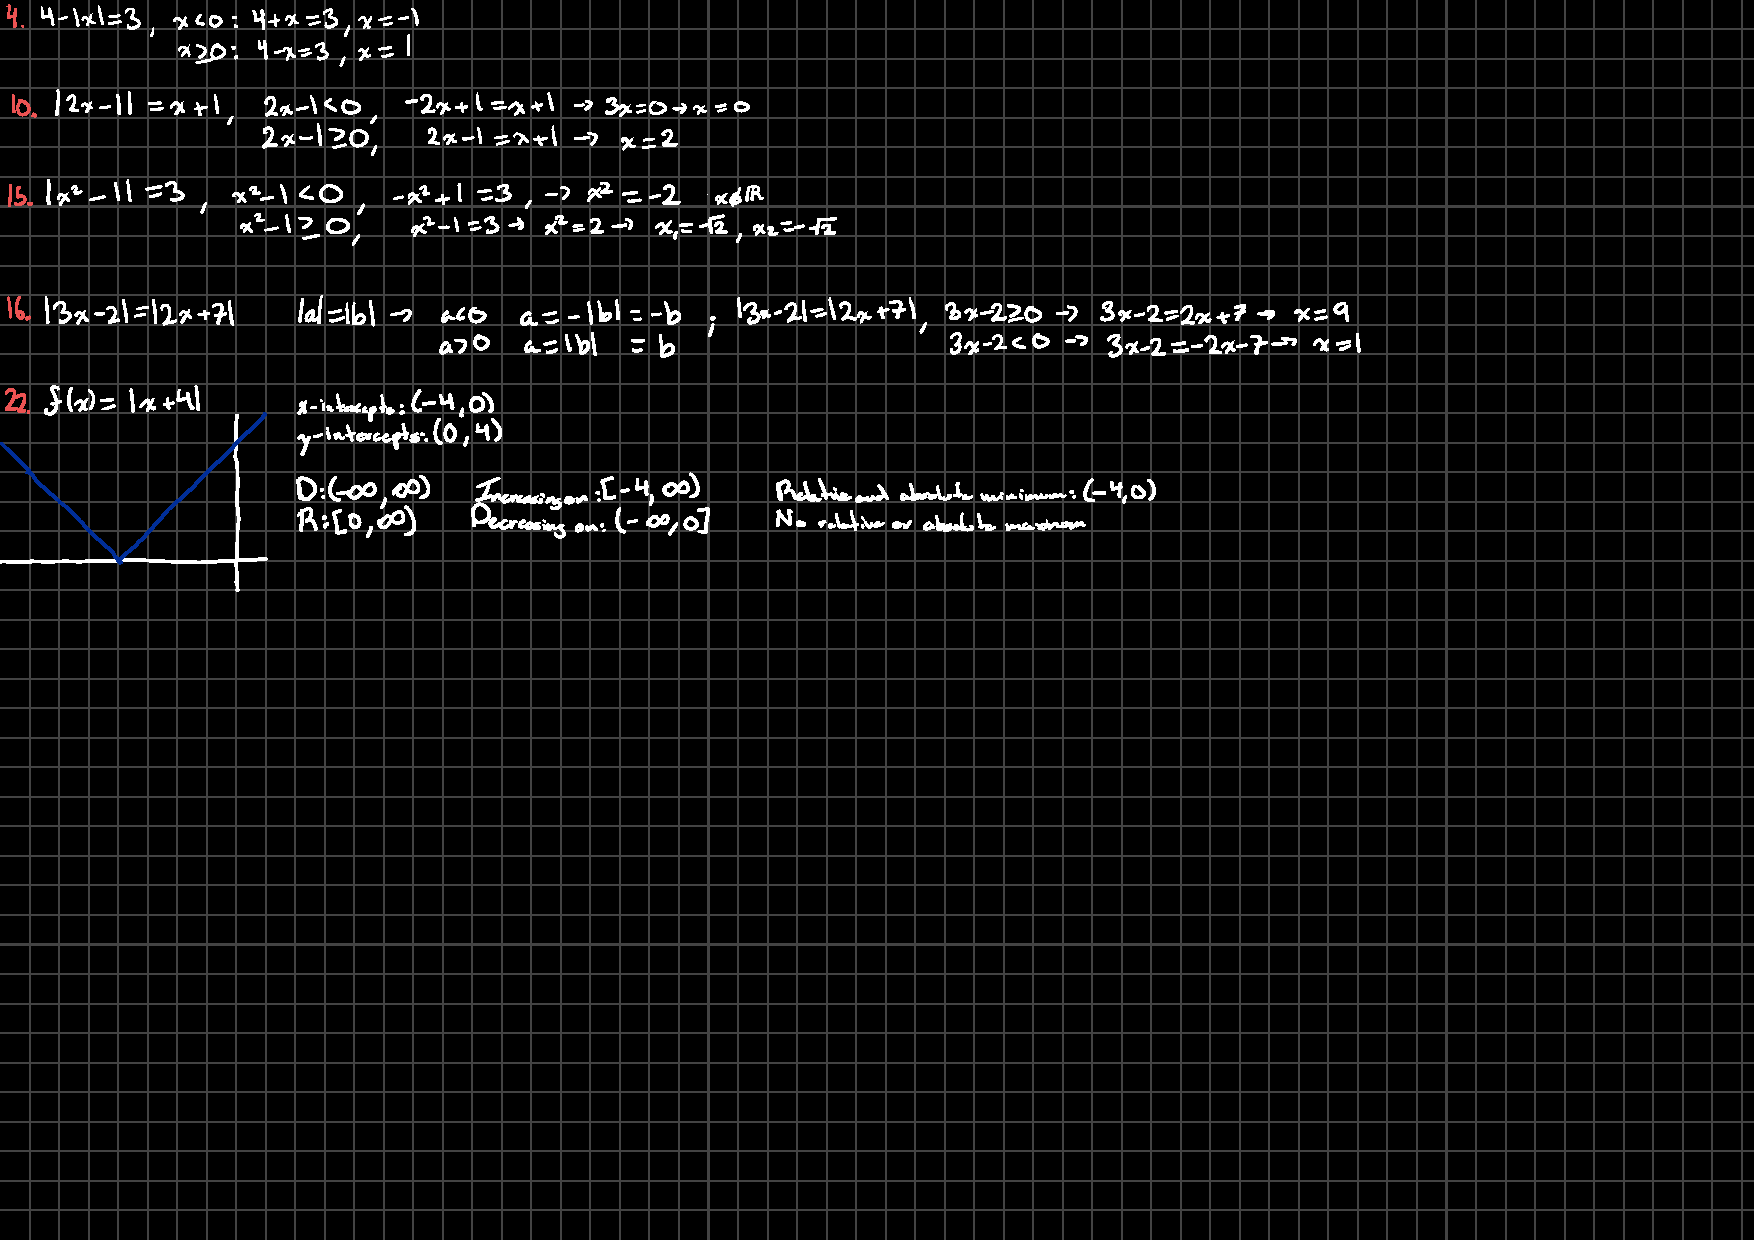
\includepdf[pages=-]{Exercises/02_Linear_and_Quadratic_Functions/02_Absolute_Value_Functions.pdf}
